
\section{MLflow}

Elk van de Proof of Concepts bevat MLflow. Zoals besproken in Sectie~\ref{subsec:mlflow} heeft dit framework veel functionaliteiten. Voor deze Proof of Concepts worden vooral de parameters van het model, de resultaten van de training en de resultaten van de evaluatie bijgehouden. Dit wordt \textit{Experiment Tracking} genoemd en maakt het mogelijk om experimenten bij te houden.

\subsection{Installatie}

Alvorens MLflow gebruikt kan worden, moet het geïnstalleerd worden. Dit kan met behulp van \texttt{pip}:

\begin{minted}{bash}
    pip install MLflow
\end{minted}

Vervolgens kan MLflow geïmporteerd worden in de Python-code met behulp van de volgende lijnen code:

\begin{minted}{python}
    import MLflow
    import MLflow.keras
\end{minted}

Nadat MLflow geïmporteerd is, moeten alle parameters in de code aangepast worden. Zo stuurt het de resultaten naar de juiste server en worden de juiste resultaten bijgehouden. De parameters die aangepast moeten worden zijn als volgt:

\begin{itemize}
    \item \textbf{Parameter Logging}: Het commando hiervoor is \texttt{mflow().log\_param}. Dit houdt alle parameters van het model bij, zoals het aantal epochs of de batchgrootte.
    \item \textbf{Metric Logging}: Tijdens het trainen van het model zal MLflow belangrijke resulaten bijhouden, zoals de nauwkeurigheid en het verlies van het model. Dit wordt aan de hand van \texttt{MLflow.log\_metric()} bijgehouden. Deze metrics worden voor elke epoch in het trainingsproces bijgehouden om het verloop van de training te analyseren.
\end{itemize}

Als MLflow geïnstalleerd is en alle parameters correct zijn ingesteld, kan de lokale server worden opgestart met het volgende commando:

\begin{minted}{bash}
    MLflow server --host 127.0.0.1 --port 8080
\end{minted}

Dit commando heeft de volgende parameters:

\begin{itemize}
    \item \texttt{host}: voor het instellen van het ip addres voor de lokale server.
    \item \texttt{port}: voor het instellen van de poort van de lokale server.
\end{itemize}

Nadat de server opgestart is, kan naar het ingestelde adres worden genavigeerd in een webbrowser om het dashboard te zien. Het dashboard van MLflow geeft de resulaten van alle pipelines weer, zie het voorbeeld in Figuur~\ref{fig:MLflow_dashboard}.

\begin{figure}[h]
    \centering
    \includegraphics[width=0.9\linewidth]{graphics/MLflow_dashboard.PNG}
    \caption{Voorbeeld van het MLflow dashboard}
    \label{fig:MLflow_dashboard}
\end{figure}

In het menu zijn de verschillende projecten te zien. Als een project geselecteerd is, kunnen alle uitvoeringen worden bekeken, zoals te zien is in Figuur~\ref{fig:MLflow_runs}.

\begin{figure}[h]
    \centering
    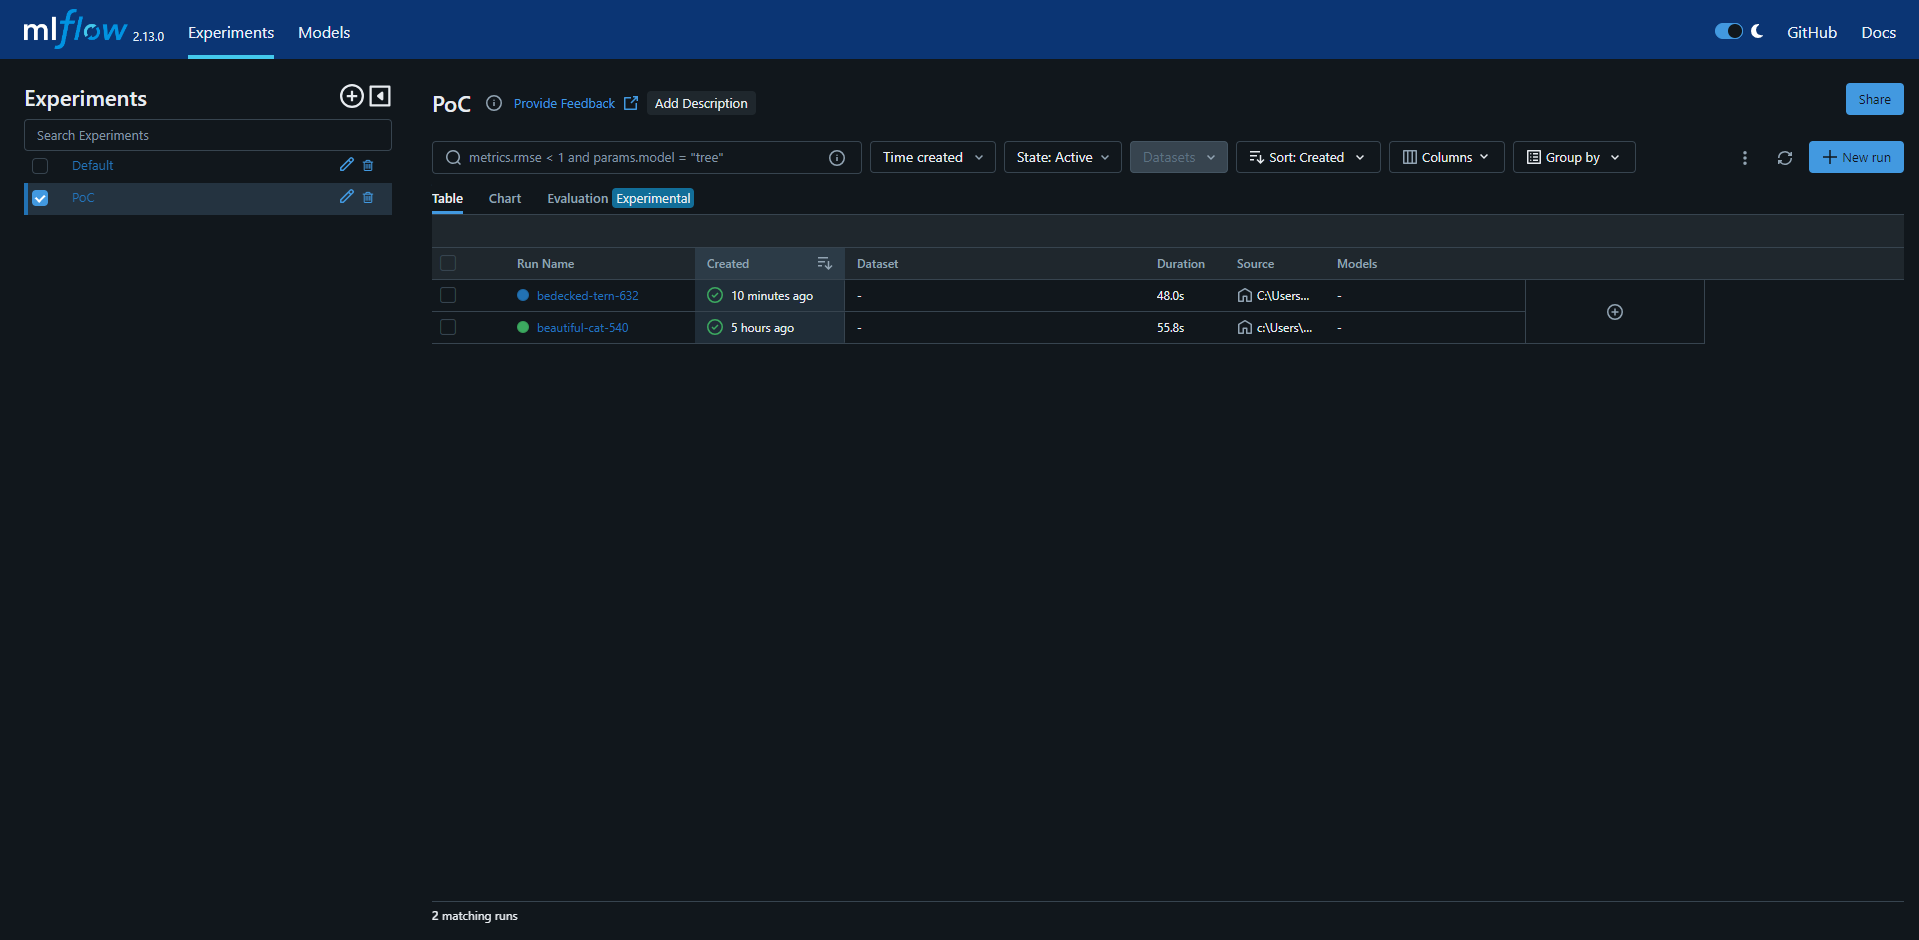
\includegraphics[width=0.9\linewidth]{graphics/MLflow_Runs.PNG}
    \caption{Verschillende pipelines in MLflow}
    \label{fig:MLflow_runs}
\end{figure}

Er kan ook een uitvoering worden geselecteerd, waardoor er meer in detail kan worden gekeken. Hierbij worden de gedefinieerde parameters en de prestatie van de uitvoering weergegeven. Figuur~\ref{fig:MLflow_informatie} toont hoe deze pagina eruit ziet:

\begin{figure}[h]
    \centering
    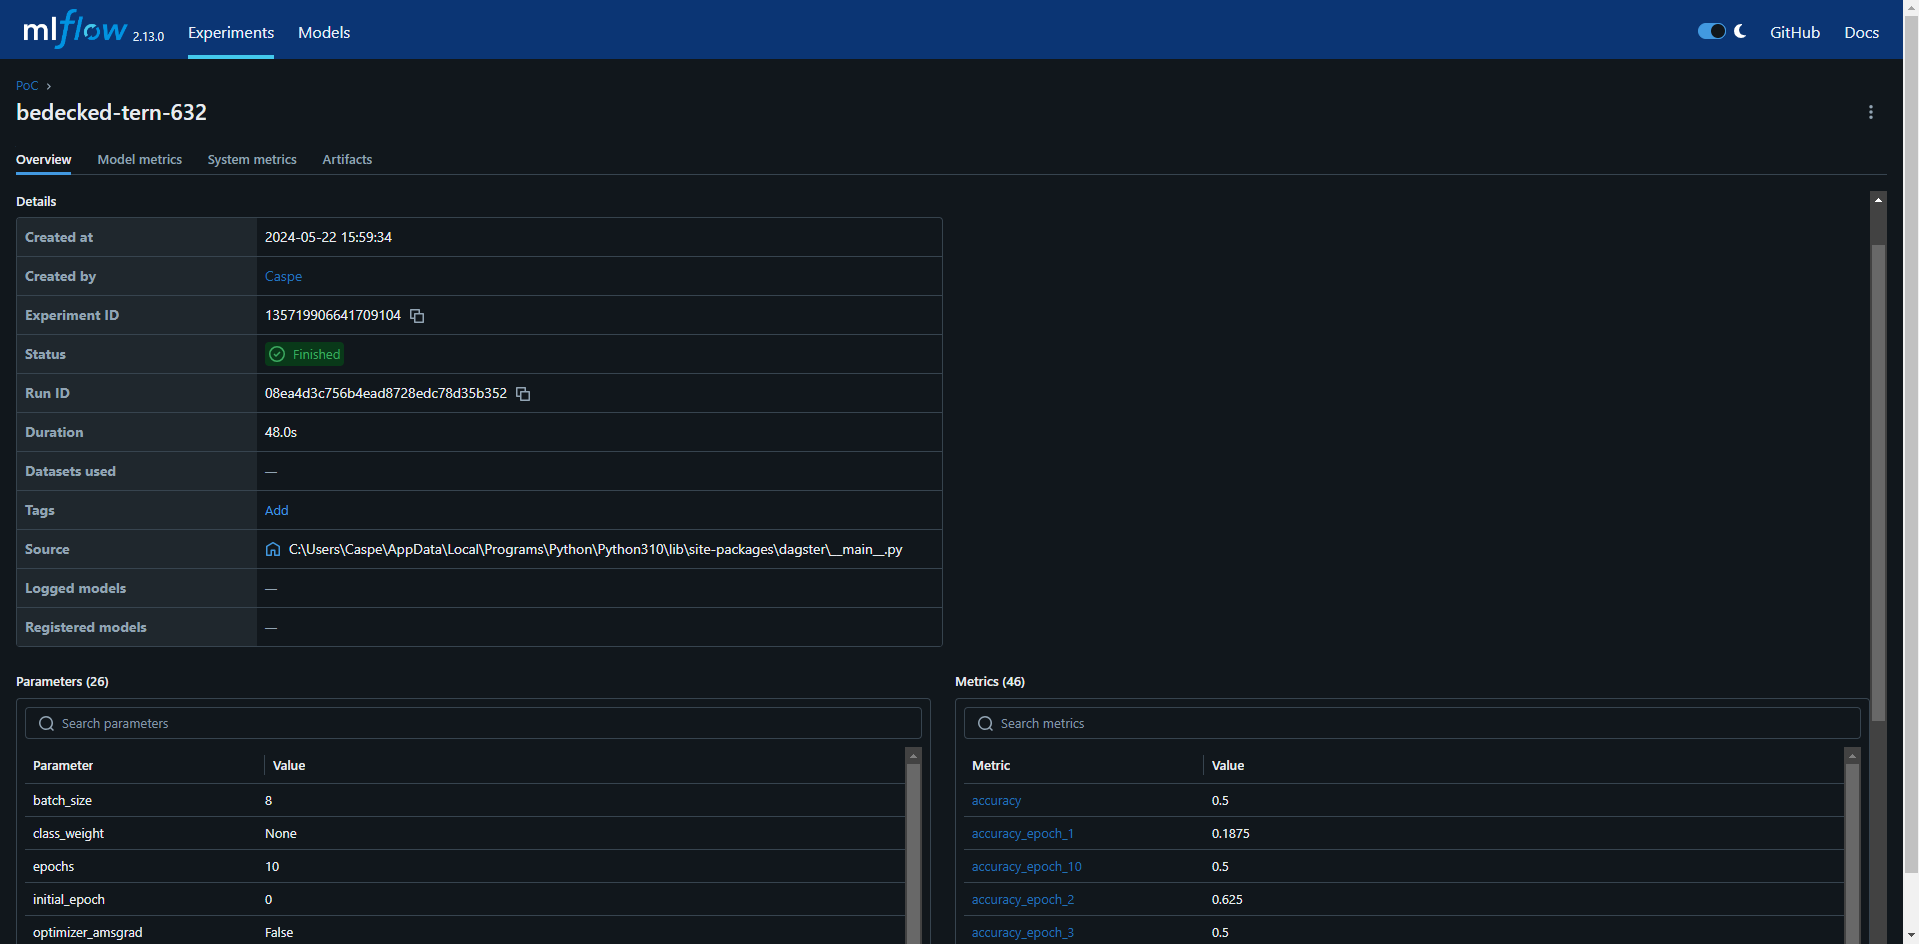
\includegraphics[width=0.9\linewidth]{graphics/MLflow_Information.PNG}
    \caption{Gedetaileerde pagina van pipeline uitvoering in MLflow}
    \label{fig:MLflow_informatie}
\end{figure}

Verder kunnen ook de grafieken worden bekeken die laten zien hoe het model heeft gepresteerd tijdens het trainen en evalueren, zoals te zien is in Figuur~\ref{fig:MLflow_graph}.

\begin{figure}[h]
    \centering
    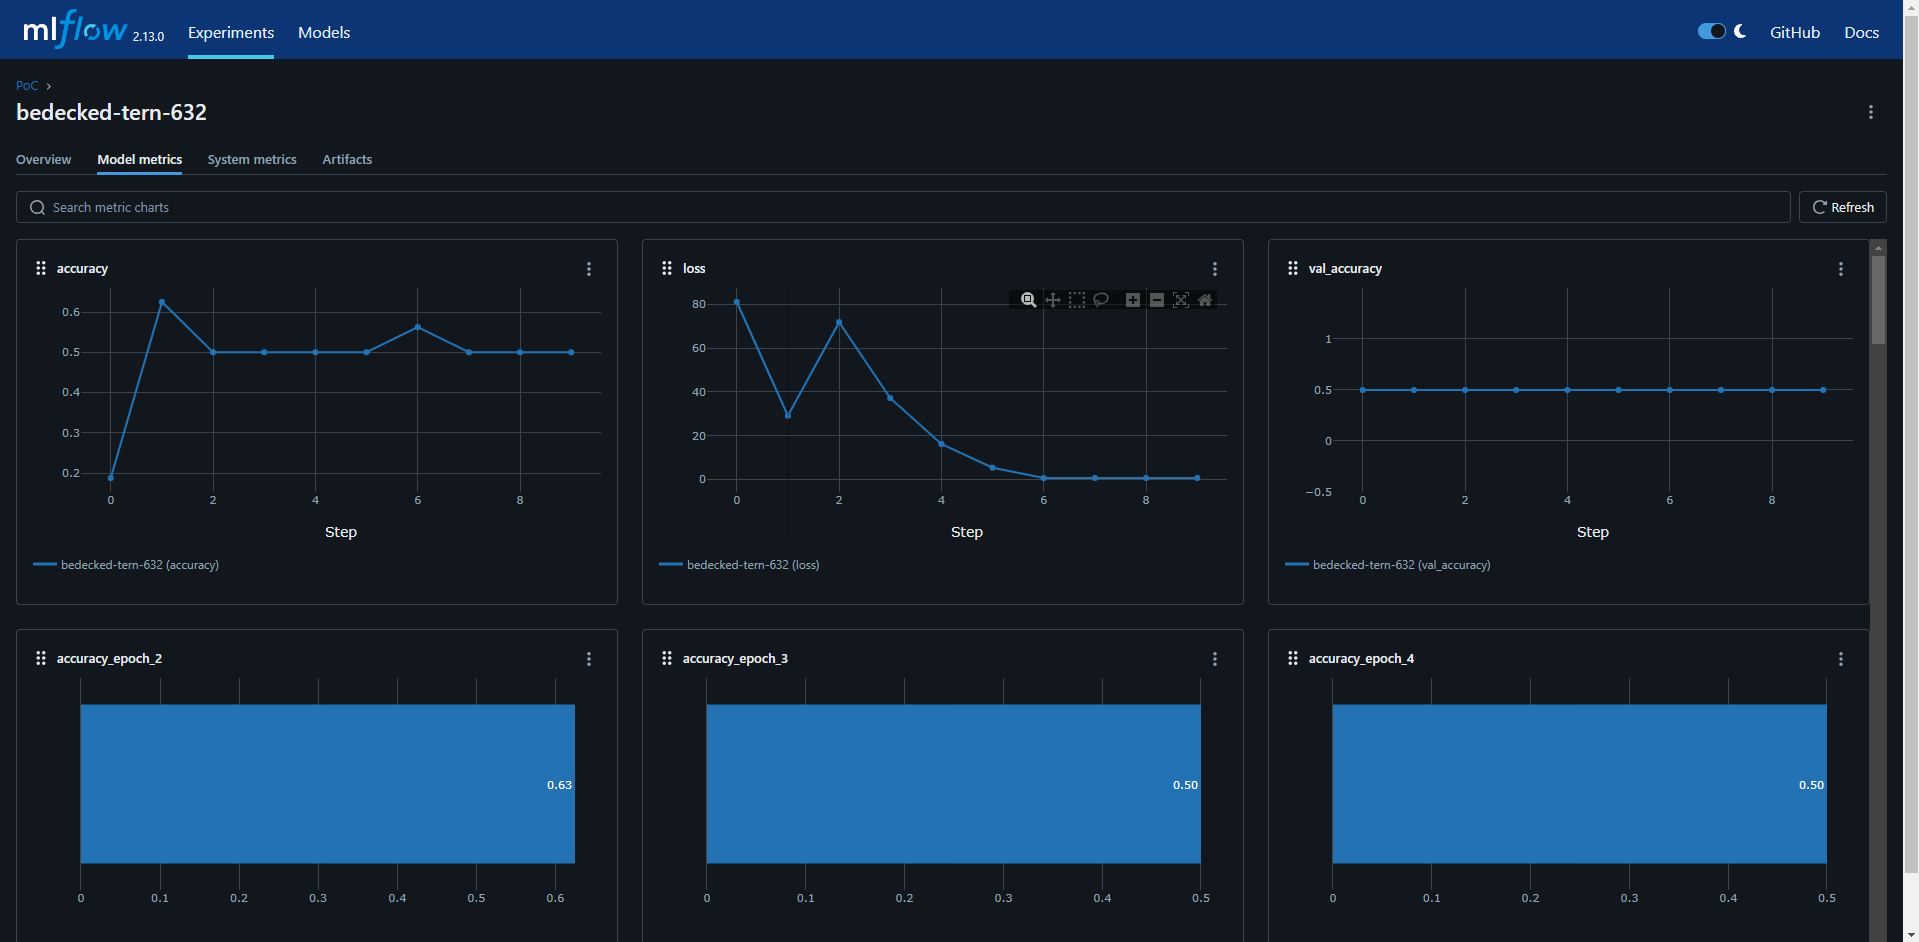
\includegraphics[width=0.9\linewidth]{graphics/mlflow_Graph.PNG}
    \caption{Grafieken van pipeline uitvoering in MLflow}
    \label{fig:MLflow_graph}
\end{figure}